\documentclass{beamer}

\usetheme{Madrid}
\usecolortheme{default}
%\setbeamercolor{block body}{bg = white}
%\setbeamercolor{block title}{bg = blue!30, fg = black}

\newif\ifbeamer
\beamerfalse
\let\oldemptyset\emptyset
\let\emptyset\varnothing
%\let\phi\varphi
\let\epsilon\varepsilon

\usepackage{amssymb}
\usepackage{amsfonts}
\usepackage{amsthm}
\usepackage{amsmath}
\usepackage{mathtools}
\usepackage{bbm}
\usepackage{bussproofs}
\usepackage{verbatim}
\usepackage{mathrsfs}
\usepackage{tikz, tikz-cd}
%\usepackage{fullpage}
\usepackage[all,2cell]{xy}
\xyoption{2cell}
\usepackage{ stmaryrd } %For power series ring brackets
%\usepackage{todonotes}
%\ue[style = numeric]{biblatex}
%\addbibresource{ThesisBib.bib}



%TikzSet
\tikzset{%
	symbol/.style={%
		draw=none,
		every to/.append style={%
			edge node={node [sloped, allow upside down, auto=false]{$#1$}}}
	}
}

%Tikz Libraries
\usetikzlibrary{matrix,arrows}

\newtheorem{COMMAND}{NameToAppear}

\DeclareMathOperator{\command}{definition}
\DeclareMathOperator{\SumZeroInf}{\sum_{\mathnormal{k} = 0}^{\infty}}

%Theorem Environments
%\newtheorem{Theorem}{Theorem}
%\newtheorem{Lemma}[Theorem]{Lemma}
%\newtheorem{Corollary}[Theorem]{Corollary}
%\newtheorem{conjecture}[Theorem]{Conjecture}
%\newtheorem{claim}[Theorem]{Claim}
%\newtheorem{proposition}[Theorem]{Proposition}
%\newtheorem{lemma}[Theorem]{Lemma}
%\newtheorem{corollary}[Theorem]{Corollary}

%Definition Style Theorem Environments
%\theoremstyle{definition}
%\newtheorem{example}[Theorem]{Example}
%\newtheorem{remark}[Theorem]{Remark}
%\newtheorem{definition}[Theorem]{Definition}
%\newtheorem{hypo}[Theorem]{Hypothesis}
%\newtheorem{goal}[Theorem]{Goal}
%\newtheorem{exercise}{Exercise}

%Scriptabet
\DeclareMathOperator{\Ascr}{\mathscr{A}}
\DeclareMathOperator{\Bscr}{\mathscr{B}}
\DeclareMathOperator{\Cscr}{\mathscr{C}}
\DeclareMathOperator{\Dscr}{\mathscr{D}}
\DeclareMathOperator{\Escr}{\mathscr{E}}
\DeclareMathOperator{\Fscr}{\mathscr{F}}
\DeclareMathOperator{\Gscr}{\mathscr{G}}
\DeclareMathOperator{\Hscr}{\mathscr{H}}
\DeclareMathOperator{\Iscr}{\mathscr{I}}
\DeclareMathOperator{\Jscr}{\mathscr{J}}
\DeclareMathOperator{\Kscr}{\mathscr{K}}
\DeclareMathOperator{\Lscr}{\mathscr{L}}
\DeclareMathOperator{\Mscr}{\mathscr{M}}
\DeclareMathOperator{\Nscr}{\mathscr{N}}
\DeclareMathOperator{\Oscr}{\mathscr{O}}
\DeclareMathOperator{\Pscr}{\mathscr{P}}
\DeclareMathOperator{\Qscr}{\mathscr{Q}}
\DeclareMathOperator{\Rscr}{\mathscr{R}}
\DeclareMathOperator{\Sscr}{\mathscr{S}}
\DeclareMathOperator{\Tscr}{\mathscr{T}}
\DeclareMathOperator{\Uscr}{\mathscr{U}}
\DeclareMathOperator{\Vscr}{\mathscr{V}}
\DeclareMathOperator{\Wscr}{\mathscr{W}}
\DeclareMathOperator{\Xscr}{\mathscr{X}}
\DeclareMathOperator{\Yscr}{\mathscr{Y}}
\DeclareMathOperator{\Zscr}{\mathscr{Z}}

%Blackboardboldtabet
\DeclareMathOperator{\Abb}{\mathbb{A}}
%\DeclareMathOperator{\Bbb}{\mathbb{B}}
\DeclareMathOperator{\Cbb}{\mathbb{C}}
\DeclareMathOperator{\Dbb}{\mathbb{D}}
\DeclareMathOperator{\Ebb}{\mathbb{E}}
\DeclareMathOperator{\Fbb}{\mathbb{F}}
\DeclareMathOperator{\Gbb}{\mathbb{G}}
\DeclareMathOperator{\Hbb}{\mathbb{H}}
\DeclareMathOperator{\Ibb}{\mathbb{I}}
\DeclareMathOperator{\Jbb}{\mathbb{J}}
\DeclareMathOperator{\Kbb}{\mathbb{K}}
\DeclareMathOperator{\Lbb}{\mathbb{L}}
\DeclareMathOperator{\Mbb}{\mathbb{M}}
\DeclareMathOperator{\Nbb}{\mathbb{N}}
\DeclareMathOperator{\Obb}{\mathbb{O}}
\DeclareMathOperator{\Pbb}{\mathbb{P}}
\DeclareMathOperator{\Qbb}{\mathbb{Q}}
\DeclareMathOperator{\Rbb}{\mathbb{R}}
\DeclareMathOperator{\Sbb}{\mathbb{S}}
\DeclareMathOperator{\Tbb}{\mathbb{T}}
\DeclareMathOperator{\Ubb}{\mathbb{U}}
\DeclareMathOperator{\Vbb}{\mathbb{V}}
\DeclareMathOperator{\Wbb}{\mathbb{W}}
\DeclareMathOperator{\Xbb}{\mathbb{X}}
\DeclareMathOperator{\Ybb}{\mathbb{Y}}
\DeclareMathOperator{\Zbb}{\mathbb{Z}}

%Calphabet
\DeclareMathOperator{\Acal}{\mathcal{A}}
\DeclareMathOperator{\Bcal}{\mathcal{B}}
\DeclareMathOperator{\Ccal}{\mathcal{C}}
\DeclareMathOperator{\Dcal}{\mathcal{D}}
\DeclareMathOperator{\Ecal}{\mathcal{E}}
\DeclareMathOperator{\Fcal}{\mathcal{F}}
\DeclareMathOperator{\Gcal}{\mathcal{G}}
\DeclareMathOperator{\Hcal}{\mathcal{H}}
\DeclareMathOperator{\Ical}{\mathcal{I}}
\DeclareMathOperator{\Jcal}{\mathcal{J}}
\DeclareMathOperator{\Kcal}{\mathcal{K}}
\DeclareMathOperator{\Lcal}{\mathcal{L}}
\DeclareMathOperator{\Mcal}{\mathcal{M}}
\DeclareMathOperator{\Ncal}{\mathcal{N}}
\DeclareMathOperator{\Ocal}{\mathcal{O}}
\DeclareMathOperator{\Pcal}{\mathcal{P}}
\DeclareMathOperator{\Qcal}{\mathcal{Q}}
\DeclareMathOperator{\Rcal}{\mathcal{R}}
\DeclareMathOperator{\Scal}{\mathcal{S}}
\DeclareMathOperator{\Tcal}{\mathcal{T}}
\DeclareMathOperator{\Ucal}{\mathcal{U}}
\DeclareMathOperator{\Vcal}{\mathcal{V}}
\DeclareMathOperator{\Wcal}{\mathcal{W}}
\DeclareMathOperator{\Xcal}{\mathcal{X}}
\DeclareMathOperator{\Ycal}{\mathcal{Y}}
\DeclareMathOperator{\Zcal}{\mathcal{Z}}

%Fraktabet
\DeclareMathOperator{\Afrak}{\mathfrak{A}}
\DeclareMathOperator{\afrak}{\mathfrak{a}}
\DeclareMathOperator{\Bfrak}{\mathfrak{B}}
\DeclareMathOperator{\bfrak}{\mathfrak{b}}
\DeclareMathOperator{\Cfrak}{\mathfrak{C}}
\DeclareMathOperator{\cfrak}{\mathfrak{c}}
\DeclareMathOperator{\Dfrak}{\mathfrak{D}}
\DeclareMathOperator{\dfrak}{\mathfrak{d}}
\DeclareMathOperator{\Efrak}{\mathfrak{E}}
\DeclareMathOperator{\efrak}{\mathfrak{e}}
\DeclareMathOperator{\Ffrak}{\mathfrak{F}}
\DeclareMathOperator{\ffrak}{\mathfrak{f}}
\DeclareMathOperator{\Gfrak}{\mathfrak{G}}
\DeclareMathOperator{\gfrak}{\mathfrak{g}}
\DeclareMathOperator{\Hfrak}{\mathfrak{H}}
\DeclareMathOperator{\hfrak}{\mathfrak{h}}
\DeclareMathOperator{\Ifrak}{\mathfrak{I}}
\DeclareMathOperator{\ifrak}{\mathfrak{i}}
\DeclareMathOperator{\Jfrak}{\mathfrak{J}}
\DeclareMathOperator{\jfrak}{\mathfrak{j}}
\DeclareMathOperator{\Kfrak}{\mathfrak{K}}
\DeclareMathOperator{\kfrak}{\mathfrak{k}}
\DeclareMathOperator{\Lfrak}{\mathfrak{L}}
\DeclareMathOperator{\lfrak}{\mathfrak{l}}
\DeclareMathOperator{\Mfrak}{\mathfrak{M}}
\DeclareMathOperator{\mfrak}{\mathfrak{m}}
\DeclareMathOperator{\Nfrak}{\mathfrak{N}}
\DeclareMathOperator{\nfrak}{\mathfrak{n}}
\DeclareMathOperator{\Ofrak}{\mathfrak{O}}
\DeclareMathOperator{\ofrak}{\mathfrak{o}}
\DeclareMathOperator{\Pfrak}{\mathfrak{P}}
\DeclareMathOperator{\pfrak}{\mathfrak{p}}
\DeclareMathOperator{\Qfrak}{\mathfrak{Q}}
\DeclareMathOperator{\qfrak}{\mathfrak{q}}
\DeclareMathOperator{\Rfrak}{\mathfrak{R}}
\DeclareMathOperator{\rfrak}{\mathfrak{r}}
\DeclareMathOperator{\Sfrak}{\mathfrak{S}}
\DeclareMathOperator{\sfrak}{\mathfrak{s}}
\DeclareMathOperator{\Tfrak}{\mathfrak{T}}
\DeclareMathOperator{\tfrak}{\mathfrak{t}}
\DeclareMathOperator{\Ufrak}{\mathfrak{U}}
\DeclareMathOperator{\ufrak}{\mathfrak{u}}
\DeclareMathOperator{\Vfrak}{\mathfrak{V}}
\DeclareMathOperator{\vfrak}{\mathfrak{v}}
\DeclareMathOperator{\Wfrak}{\mathfrak{W}}
\DeclareMathOperator{\wfrak}{\mathfrak{w}}
\DeclareMathOperator{\Xfrak}{\mathfrak{X}}
\DeclareMathOperator{\xfrak}{\mathfrak{x}}
\DeclareMathOperator{\Yfrak}{\mathfrak{Y}}
\DeclareMathOperator{\yfrak}{\mathfrak{y}}
\DeclareMathOperator{\Zfrak}{\mathfrak{Z}}
\DeclareMathOperator{\zfrak}{\mathfrak{z}}

%Math Operators and Shorthands
%\DeclareMathOperator{\hfrak}{\mathfrak{h}}
\DeclareMathOperator{\Var}{\underline{Var}}
\DeclareMathOperator{\quo}{\mathsf{quo}}
\DeclareMathOperator{\QCat}{\underline{QCat}}
\DeclareMathOperator{\fQCat}{\mathfrak{QCat}}
\DeclareMathOperator{\hQCat}{\mathfrak{hQCat}}
\DeclareMathOperator{\sk}{sk}
\DeclareMathOperator{\skel}{skel}
\DeclareMathOperator{\cosk}{cosk}
\DeclareMathOperator{\coskel}{coskel}
\DeclareMathOperator{\Nerve}{Ner}
\DeclareMathOperator{\infCat}{\underline{QCat}}
\DeclareMathOperator{\QCoh}{\mathbf{QCoh}}
\DeclareMathOperator{\Shv}{\mathbf{Shv}}
\DeclareMathOperator{\Rel}{\mathbf{Rel}}
\DeclareMathOperator{\mor}{Mor}
\DeclareMathOperator{\id}{id}
\DeclareMathOperator{\ob}{Ob}
\DeclareMathOperator{\Hom}{Hom}
\DeclareMathOperator{\Ker}{Ker}
\DeclareMathOperator{\End}{End}
\DeclareMathOperator{\Tor}{Tor}
\DeclareMathOperator{\sSet}{[\underline{\Delta}^{\operatorname{op}},\Set]}
\DeclareMathOperator{\SSS}{\mathbb{S}}
\DeclareMathOperator{\Set}{\underline{Set}}
\DeclareMathOperator{\col}{Col}
\DeclareMathOperator{\row}{Row}
\DeclareMathOperator{\ord}{ord}
\DeclareMathOperator{\Span}{span}
\DeclareMathOperator{\gln}{GL}
\DeclareMathOperator{\aut}{Aut}
\DeclareMathOperator{\mat}{Mat}
\DeclareMathOperator{\Nx}{\mathbb{N}^{\times}}
\DeclareMathOperator{\tran}{T}
\DeclareMathOperator{\Ann}{Ann}
\DeclareMathOperator{\Topos}{\mathbf{Topos}}
\DeclareMathOperator{\R}{\mathbb{R}}
\DeclareMathOperator{\C}{\mathbb{C}}
\DeclareMathOperator{\Z}{\mathbb{Z}}
\DeclareMathOperator{\N}{\mathbb{N}}
\DeclareMathOperator{\card}{card}
\DeclareMathOperator{\DVect}{\mathbf{D-Vect}}
\DeclareMathOperator{\Gal}{Gal}
\DeclareMathOperator{\Br}{Br}
\DeclareMathOperator{\Cofree}{Cofree}
\DeclareMathOperator{\ann}{Ann}
\DeclareMathOperator{\KAlg}{\mathbf{K-Alg}}
\DeclareMathOperator{\LAlg}{\mathbf{L-Alg}}
\DeclareMathOperator{\KVect}{\mathbf{K-Vect}}
\DeclareMathOperator{\PP}{\mathbb{P}}
\DeclareMathOperator{\RMod}{\mathbf{R-Mod}}
\DeclareMathOperator{\ModR}{\mathbf{Mod-R}}
\DeclareMathOperator{\Rng}{\mathbf{Rng}}
\DeclareMathOperator{\Ring}{\mathbf{Ring}}
\DeclareMathOperator{\FSch}{\mathbf{FSch}}
\DeclareMathOperator{\Cring}{\mathbf{Cring}}
\DeclareMathOperator{\Crng}{\mathbf{Crng}}
\DeclareMathOperator{\Ab}{\mathbf{Ab}}
\DeclareMathOperator{\Grp}{\mathbf{Grp}}
\DeclareMathOperator{\Q}{\mathbb{Q}}
\DeclareMathOperator{\FpAlg}{\mathbb{F}_{\mathnormal{p}}\mathbff{-Alg}}
\DeclareMathOperator{\kAlg}{\mathnormal{k}\mathbf{-Alg}}
\DeclareMathOperator{\im}{Im}
\DeclareMathOperator{\Ext}{Ext}
\DeclareMathOperator{\cd}{cd}
\DeclareMathOperator{\Char}{char}
\DeclareMathOperator{\colim}{colim}
\DeclareMathOperator{\fix}{Fix}
\DeclareMathOperator{\algextK}{\mathbf{AlgExt(K)}}
\DeclareMathOperator{\finextK}{\mathbf{FinExt(K)}}
\DeclareMathOperator{\extK}{\mathbf{Ext(K)}}
\DeclareMathOperator{\CalO}{\mathcal{O}}
\DeclareMathOperator{\nil}{\mathfrak{nil}}
\DeclareMathOperator{\Spec}{Spec}
\DeclareMathOperator{\Sch}{\mathbf{Sch}}
%\DeclareMathOperator{\Ccat}{\mathfrak{C}}
\DeclareMathOperator{\Dom}{Dom}
\DeclareMathOperator{\true}{true}
\DeclareMathOperator{\FinSet}{\mathbf{FinSet}}
\DeclareMathOperator{\CalF}{\mathcal{F}}
\DeclareMathOperator{\AffSch}{\mathbf{AffSch}}
%\DeclareMathOperator{\Dfrak}{\mathfrak{D}}
\DeclareMathOperator{\Poset}{\mathbf{Poset}}
\DeclareMathOperator{\Free}{Free}
\DeclareMathOperator{\Forget}{Forget}
\DeclareMathOperator{\Cat}{\underline{Cat}}
\DeclareMathOperator{\Digraph}{\mathbf{Digraph}}
\DeclareMathOperator{\Fun}{\mathbf{Fun}}
\DeclareMathOperator{\Nat}{\mathbf{Nat}}
\DeclareMathOperator{\Aut}{Aut}
\DeclareMathOperator{\Field}{\mathbf{Field}}
\DeclareMathOperator{\Fix}{Fix}
\DeclareMathOperator{\FinRel}{\mathbf{FinRel}}
\DeclareMathOperator{\BoolMat}{\mathbf{BoolMat}}
\DeclareMathOperator{\CalE}{\mathcal{E}}
\DeclareMathOperator{\hC}{h\mathfrak{C}}
\DeclareMathOperator{\Top}{\mathbf{Top}}
\DeclareMathOperator{\hTop}{h\mathbf{Top}}
\DeclareMathOperator{\ChRMod}{\mathbf{Ch}_{n \geq 0}(\mathbf{R-Mod})}
\DeclareMathOperator{\Coker}{Coker}
\DeclareMathOperator{\coker}{coker}
%\DeclareMathOperator{\Afrak}{\mathfrak{A}}
\DeclareMathOperator{\KMod}{\mathbf{K-Mod}}
\DeclareMathOperator{\KModK}{\mathbf{K-Mod-K}}
\DeclareMathOperator{\Mon}{\mathbf{Mon}}
\DeclareMathOperator{\Frop}{Fro_{\mathnormal{p}}}
\DeclareMathOperator{\ring}{\mathbf{ring}}
\DeclareMathOperator{\Fp}{\mathbb{F}_{\mathnormal{p}}}
\DeclareMathOperator{\Gr}{Gr}
\DeclareMathOperator{\ASch}{\mathbf{AffSch}}
\DeclareMathOperator{\Sym}{Sym}
\DeclareMathOperator{\RAlg}{\mathbf{\mathnormal{R}-Alg}}
\DeclareMathOperator{\RAlgFl}{\mathbf{\mathnormal{R}-Alg}_{Fl}}
\DeclareMathOperator{\PsiRERing}{\mathbf{{\Psi_{R,E}}-Ring}}
\DeclareMathOperator{\LambdaRERing}{\mathbf{\mathnormal{\Lambda_{R,E}}-Ring}}
\DeclareMathOperator{\Frqe}{Fr_{\mathnormal{q_{e}}}}
\DeclareMathOperator{\LocRingSpac}{\mathbf{LRS}}
\DeclareMathOperator{\Spf}{Spf}
\DeclareMathOperator{\Codom}{Codom}
\DeclareMathOperator{\codom}{Codom}
%\DeclareMathOperator{\pfrak}{\mathfrak{p}}
%\DeclareMathOperator{\frakX}{\mathfrak{X}}
%\DeclareMathOperator{\frakY}{\mathfrak{Y}}
%\DeclareMathOperator{\qfrak}{\mathfrak{q}}
\DeclareMathOperator{\Iso}{\mathcal{I}so}
\DeclareMathOperator{\A}{\mathbb{A}}
\DeclareMathOperator{\AFJ}{\mathcal{A}_{\mathnormal{F}}^{\mathnormal{J}}}
\DeclareMathOperator{\Fi}{Fi}
\DeclareMathOperator{\op}{op}
\DeclareMathOperator{\Ccat}{\mathscr{C}}
\DeclareMathOperator{\Dcat}{\mathscr{D}}
\DeclareMathOperator{\Iner}{Inert}
\DeclareMathOperator{\G}{\mathbb{G}}
\DeclareMathOperator{\QAGrp}{\mathbf{QAlgGrp}}
\DeclareMathOperator{\PAGrp}{\mathbf{ProAlgGrp}}
\DeclareMathOperator{\GL}{GL}
\DeclareMathOperator{\ProfAGrp}{\mathbf{ProAb}}
\DeclareMathOperator{\SL}{SL}
\DeclareMathOperator{\Ev}{Ev}
\DeclareMathOperator{\NEv}{NEv}
\DeclareMathOperator{\Frob}{Frob}
\DeclareMathOperator{\Per}{\mathbf{Per}}
\DeclareMathOperator{\IC}{IC}
\DeclareMathOperator{\supp}{supp}
\DeclareMathOperator{\naive}{\textnormal{na{\"i}ve}}
\DeclareMathOperator{\trace}{trace}
\DeclareMathOperator{\ev}{eval}
\DeclareMathOperator{\Sf}{\underline{Sf}}
\DeclareMathOperator{\GVar}{\mathnormal{G}-\mathbf{Var}}
\DeclareMathOperator{\calL}{\mathcal{L}}
\DeclareMathOperator{\modH}{\mathbf{Mod}_{\C-f.d.}-\Hcal}
\DeclareMathOperator{\modHow}{\mathbf{Mod}_{\C-f.d.}^{\mathnormal{\omega}}-\Hcal}
\DeclareMathOperator{\AdRep}{\mathbf{AdRep}}
\DeclareMathOperator{\modHoh}{\mathbf{Mod}_{\C-f.d.}^{\mathnormal{\omega_{\mathnormal{h}}}}-\mathbb{H}}
\DeclareMathOperator{\uGamma}{{}_{\Gamma}}
\DeclareMathOperator{\mult}{mult}
\DeclareMathOperator{\CVect}{\mathbb{C}-\mathbf{Vect}}
\DeclareMathOperator{\OXMod}{\mathcal{O}_{\mathnormal{X}}-\mathbf{Mod}}
\DeclareMathOperator{\OYMod}{\mathcal{O}_{\mathnormal{Y}}-\mathbf{Mod}}
%\DeclareMathOperator{\Ch}{\mathbf{Ch}}
\DeclareMathOperator{\coim}{Coim}
\DeclareMathOperator{\Add}{\mathbf{Add}}
\DeclareMathOperator{\per}{{}^{p}}
\DeclareMathOperator{\GMod}{\matnormal{G}-\mathbf{Mod}}
\DeclareMathOperator{\DbcGX}{D_{c,\mathnormal{G}}^{b}(\mathnormal{X},\overline{\mathbb{Q}}_{\ell})}
\DeclareMathOperator{\DbcGXGamma}{D_{c}^{b}(\quot{X}{\Gamma},\overline{\mathbb{Q}}_{\ell})}
\DeclareMathOperator{\DbcGY}{D_{c,\mathnormal{G}}^{b}(\mathnormal{Y},\overline{\mathbb{Q}}_{\ell})}
\DeclareMathOperator{\DbcGYGamma}{D_{c}^{b}(\quot{Y}{\Gamma},\overline{\mathbb{Q}}_{\ell})}
\DeclareMathOperator{\VSet}{\mathscr{V}-\mathbf{Set}}
\DeclareMathOperator{\VAb}{\mathscr{V}-\mathbf{Ab}}
\DeclareMathOperator{\uSpan}{\underline{Span}}
\DeclareMathOperator{\uCospan}{\underline{Cospan}}
\DeclareMathOperator{\res}{res}
\DeclareMathOperator{\ran}{ran}
\DeclareMathOperator{\lan}{lan}
\DeclareMathOperator{\dgCat}{\underline{dgCat}}
\DeclareMathOperator{\dgAMod}{\underline{dgCh}(\mathnormal{A}-\underline{Mod})}
\DeclareMathOperator{\AMod}{\mathnormal{A}-\underline{Mod}}
\DeclareMathOperator{\ChAMod}{\underline{Ch}(\AMod)}                                  
\DeclareMathOperator{\GrAMod}{\underline{Gr}\AMod}
\DeclareMathOperator{\dgNer}{\Nerve_{dg}}
\DeclareMathOperator{\Ch}{\underline{Ch}}
\DeclareMathOperator{\dgCh}{\underline{dgCh}}
\DeclareMathOperator{\SfResl}{\underline{SfResl}}
\DeclareMathOperator{\fCat}{\mathfrak{Cat}}


%Let Statements
\let\oldemptyset\emptyset
\let\emptyset\varnothing
\let\epsilon\varepsilon
\let\hom\Hom

%New Commands
\newcommand{\pushoutcorner}[1][dr]{\save*!/#1+1.2pc/#1:(1,-1)@^{|-}\restore} 
\newcommand{\pullbackcorner}[1][dr]{\save*!/#1-1.2pc/#1:(-1,1)@^{|-}\restore}
\newcommand{\quot}[2]{\,_{#2}{#1}}
\newcommand{\quotd}[3]{\,_{#2}^{#3}{#1}}
\newcommand{\limAtInfty}[1]{\lim_{{#1} \to \infty}}
\newcommand{\limAtWhere}[2]{\lim_{{#1} \to {#2}}}


\UseTwocells

%Number Within Control
%\numberwithin{Theorem}{section}
%\numberwithin{exercise}{subsection}
%\numberwithin{equation}{section}


\begin{document}
\title{A \TeX{}nical Skills Workshop: Tips and Tricks}
\subtitle{How to Make \LaTeX\, Your Friend}%
\date{2021 May 11}
\author{Geoff Vooys}	

\UseTwocells
\UseAllTwocells


\frame{\titlepage}
\tableofcontents

\section{Introduction and Set Up}

\begin{frame}[fragile]\frametitle{Structure of the Talk}
\only<1->{
\begin{block}{The Outline}
\only<1>{
Over the course of the next hour we'll learn how to do \LaTeX\, stuff together! Here's the rough order we'll be doing stuff:
}
\begin{itemize}
\only<1>{	
	\item Pre-requisites and setup stuff.
	\item Learn how to type math in nice ways (this includes the underrated 
	\begin{semiverbatim}
		\\operatorname\{\}
	\end{semiverbatim} command) and hints for typesetting matrices.
	\item Learn how to make your own macros and commands.
	\item Learn how to set up bibliographies using Bib\TeX, as well as how to change stuff around as necessary. I will not be covering Bib\LaTeX (so if you want to talk about Biber just wait unitl the Q\&A).
}
\only<2>{
\item Learn how to set up figures in a document (and all the chaos around this --- by the way, it kinda sucks).
\item Learn how to reference various lemmas, theorems, propositions, figures, and equations you've set up in ways that make sense. This is to save you work later and do things like hyperlink to page and proposition numbers!
\item Depending on time: Learn about how to do stuf in Beamer and make slide shows like this with \LaTeX.
}
\end{itemize}
\end{block}
}
\end{frame}

\begin{frame}[fragile]\frametitle{Setting Up}
\only<1-3>{
\begin{block}{Hi There!}
This talk is going to be interactive and I'd like you to practice stuff as we go along! For this we'll need to be able to compile some source \TeX\, as we go, so please make sure you have a way to do this. 
\only<1>{\href{https://github.com/GeoffVooys/LaTeX-Workshop-May-2021}{There will be some small take home exercises and a text file of interest to you at my git repository that I've hyperlinked to this sentence.}}
Here are your options for TeX:
\only<2-3>{
\begin{itemize}
	\item If you want to do \LaTeX\, on your own computer I recommend using Mik\TeX\, (\url{https://miktex.org/}). For typesetting IDEs I recommend the Windows option \TeX{}Studio (\url{https://www.texstudio.org/}).
\only<3>{
	\item You can use \url{https://www.overleaf.com/} if you want to use a browser based \LaTeX\, interpreter.
}
\end{itemize}
}
\end{block}
}
\only<4>{
\begin{block}{Code Snippits}
In this talk I'll occassionally be writing \LaTeX\, code on slides for stuff to do and tricks and the like. This is done in blocks like this
\begin{semiverbatim}
\\usepackage\{amsmath\} \newline
\\usepackage\{stmarysrd\} \% For power series brackets
\end{semiverbatim}
so as to better mimic raw \TeX\, code.
\end{block}
}
\end{frame}

\section{Writing Math in \LaTeX}
\begin{frame}\frametitle{Why We Learn \LaTeX}
\only<1>{
\begin{block}{The Reasons}
While \LaTeX\, has \textbf{a lot} going for it as a superior document creation/preparation tool and as a markup language, it has a severe drawback: It is complicated to learn. For most of us there is a very good reason to fight through the learning curve:
\begin{itemize}
	\item Precise, clean, and good-looking typesetting of figures, graphics, mathematics, and mathematics-adjacent material.
\end{itemize}
\end{block}
}
\only<2>{
\begin{block}{What a .tex File Looks Like}
Before we dive right in, let's set up some language to use to discuss a .tex file. I've prepared a dummy file for you all hereTODOTODO MAKE A LINK but here's a quick run-down in case you don't want to download it:
\begin{semiverbatim}
\\documentclass\{foo\}\,\% Declares that you're writing a document of type foo. \newline
{} \newline
\% This is your preamble. Packages, settings, and commands you use/need go here. \newline
{}\newline
\\begin\{document\} \%\, This is how you tell TeX to begin the document you're typesetting.\newline
\% The writing and work you do goes here.\newline
\\end\{document\}\%\, This is how you tell TeX where the document to be typeset ends.
\end{semiverbatim}
\end{block}
}
\only<3>{
\begin{block}{Where We're Going and a First Step}
We'll begin our journey by learning the least insane of these tasks first: Typesetting mathematical formulae and expressions. For this make sure that you have a .tex document open with the code
\begin{semiverbatim}
\\documentclass\{article\}  \newline
{} \newline
\\begin\{document\} \newline
\% your article/code/math goes here\newline
\\end\{document\}
\end{semiverbatim}
typed out and ready to go.
\end{block}
}
\end{frame}
\begin{frame}\frametitle{Math Typesetting in \LaTeX}
\only<1-2>{
\begin{block}{How to Begin Typesetting Math}
	\only<1>{
We all want to typeset mathematical expressions and formulae (I can say with probability $1$ that we've all needed to type a summation
\[
\sum_{n =0}^{\infty} a_nx^n
\]
at some point), but how does \LaTeX\, know to read this as math? Because of the math packages we'll load in our preamble!
}
\only<2>{
Make sure to load the following packages in your preamble whenever you want to type math by doing the following:
\begin{semiverbatim}
\\documentclass\{foo\}\newline
{}\newline
\\usepackage\{amsmath\}\newline
\\usepackage\{amsfonts\}\newline
\\usepackage\{amssymb\}\,\%\, These three packages tell us math is happening!\newline
{} \newline
\\begin\{document\}\newline
\\end\{document\}
\end{semiverbatim}
}
\end{block}
}
\only<3-6>{
\begin{block}{Typesetting Math: The Basics}
\only<3>{
When typesetting math, there are two different modes of making \LaTeX\, output math: Inline (Math) Mode and Display Mode. Here is a quick description of the two:
\begin{itemize}
	\item Inline Mode: This is math that is done within a line and internal to a sentence or line of text. Something like ``for all $x \leq 5$'' or ``whenever $a < 0$ the ring $\R[x]/(x^2+a)$ does a thing.'' This math should usually be short and not very tall.
	\item Display Mode: This is math that is done one a line all by itself, away from the text. This is usually long, complicated, and tall math like:
	\[
	\sum_{n=0}^{\infty}\left(\frac{x^n}{n!}\right)^{2}, \qquad \prod_{\substack{p \geq 2 \\ p\,\text{prime}}}\frac{1}{1-p^{-s}}, \qquad \int_X\int_Y f(x,y)\,\mathrm{d}\nu(y)\mathrm{d}\mu(x).
	\]
\end{itemize}
}
\only<4-6>{
Some handy commands we'll also want to know for typing math are given below:
\only<4>{
\begin{itemize}
	\item The command \begin{semiverbatim}
		\\mathbb\{foo\}
	\end{semiverbatim}
gives you a letter in blackboard bold font (so long as foo is a capital letter). For example: $\Abb, \Cbb, \Rbb, \Ebb, \Xbb, \Zbb$.
\item To give terms superscripts and subscripts, when in math mode type either
\begin{semiverbatim}
foo\_\{boo\}, foo\string^\{boo\}
\end{semiverbatim}
to get either $foo_{boo}$ or $foo^{boo}$.
\end{itemize}
}
\only<5>{
\begin{itemize}
	\item The command
	\begin{semiverbatim}
		\\sum
	\end{semiverbatim}
	gives a large capital sigma for use in a summation. Giving it a subscript gives a lower limit to the sum and giving it a super script gives an upper limit to the sum. Explicitly, the code
	\begin{semiverbatim}
	\\sum\_\{foo\}\string^\{boo\}
	\end{semiverbatim}
gives
\[
\sum_{foo}^{boo}
\]
\end{itemize}
}
\only<6>{
\begin{itemize}
	\item To draw an arrow between objects (like when defining function as in $f:X \to Y$) use the command:
	\begin{semiverbatim}
		\\to
	\end{semiverbatim}
\item Fractions are given by the code
\begin{semiverbatim}
	\\frac\{foo\}\{boo\}
\end{semiverbatim}
and give you the fraction
\[
\frac{foo}{boo}.
\]
\end{itemize}
}
}
\end{block}
}
\only<7>{
\begin{block}{Inline Math}
\only<7>{
Let's begin by getting to know inline math in \LaTeX. Here are some facts:
\begin{itemize}
	\item Enter inline math mode by typing $\backslash$( and close math mode by typing $\backslash$). For example:
	\begin{semiverbatim}
	We solve the equation \\( x\string^2 + 2\\) over the complex numbers \\(\\mathbb\{C\}\\)
	\end{semiverbatim}
	\item Ideally this is for shorter math that fits in a sentence of words.
	\item This is NOT for tall math! If you have a fraction either write $a/b$ if it needs to be inline or put the fraction in display mode if it needs to be tall.
\end{itemize}
}
\end{block}
}
\only<8>{
\begin{example}
The code that gives you the line that I've typed here with the math \(asd^{-1}(1/dsa)\) is:
\begin{semiverbatim}
The code that gives you the line that I've typed here with the math \\(asd\string^\{-1\}(1/dsa)\\) is:
\end{semiverbatim}

Similarly, the code that gives the line ``I really like fractions \(a/b\) inline but not \(\frac{a}{b}\)'' is:
\begin{semiverbatim}
I really like fractions \\(a/b\\) inline but not \\(\\frac\{a\}\{b\}\\)
\end{semiverbatim}
\end{example}
}
\only<9-11>{
\begin{block}{Display Mode}
\only<9>{
Let's get to know display mode math in \LaTeX.
\begin{itemize}
	\item Enter display mode by typing $\backslash$[ and close display mode by typing $\backslash$]. For example, the code
	\begin{semiverbatim}
	My favorite function is not \newline
	\\[ \newline
	\\zeta(s) = \\sum\_\{n = 1\}\string^\{\\infty\}n\string^\{-s\}. \newline
	\\]	
\end{semiverbatim}
	gives: My favorite function is not
	\[
	\zeta(s) = \sum_{n=1}^{\infty} n^{-s}.
	\]
\end{itemize}
}
\only<10>{
\begin{itemize}
	\item Alternative ways to enter display mode: By using the environments
	\begin{semiverbatim}
		\\begin\{equation*\} \newline
		foo\newline
		\\end\{equation*\}
	\end{semiverbatim}
or, if you want your equation to have a label/number to your displayed equation,
\begin{semiverbatim}
	\\begin\{equation\}\newline
	foo \newline
	\\end\{equation\}
\end{semiverbatim}
\end{itemize}
}
\only<11>{
\begin{itemize}
	\item Display mode is best used for tall equations (things with a summation or product symbol, fractions, powers of powers of numbers, etc.) and for equations to which you explicitly need to label.
\end{itemize}
}
\end{block}	
}
\only<12>{
\begin{example}
The code that gives the expression
\[
\sum_{n=0}^{\infty} \frac{(-1)^n}{n!} = \frac{1}{e}
\]
is
\begin{semiverbatim}
\\[\newline
\\sum\_\{n=0\}\string^\{\\infty\}\\frac\{(-1)\string^n\}\{n!\} = \\frac\{1\}\{e\}\newline
\\]
\end{semiverbatim}
\end{example}
}
\end{frame}

\begin{frame}\frametitle{Practice Typesetting Math}
\begin{example}
\only<1>{
Find code to write the following:

My favorite scheme is $\Abb_{\Cbb}^{\infty}$ although $\Abb_{\Cbb}^1$ is nice too. You can define something like
\[
f(z) = \sum_{n =0}^{\infty} \frac{z^n}{n!}
\]
affine-locally on them!
}
\only<2>{
Here is some sample code:
\begin{semiverbatim}
My favorite scheme is \\(\\mathbb\{A\}\_\{\\mathbb\{C\}\}\string^\{\\infty\}\\) although \\(\\mathbb\{A\}\_\{\\mathbb\{C\}\}\string^\{1\}\\) is nice too. You can define something like \newline
\\[\newline
f(z) = \\sum\_\{n=0\}\string^\{\\infty\} \\frac\{z\string^n\}\{n!\} \newline
\\]\newline
affine-locally on them!
\end{semiverbatim}
}
\end{example}
\end{frame}

\begin{frame}\frametitle{The Last Math Typesetting Topic: left/right Delimiters}
\only<1>{
\begin{example}
	Can you figure out how to make the output
	\[
	(\sum_{n \geq 1} \frac{1}{n^2}) = \frac{\pi^2}{6}
	\]
	look nice? Note those lame parentheses on the sides of the sum: can we fix them? The answer won't surprise you!
\end{example}
}
\only<2-3>{
\begin{block}{Left/Right Delimiters}
\only<2>{
Sometimes when doing math (in display mode) we have really tall operators and stuff that go inside parentheses, brackets, braces, and other such things. Without doing some ninjitsu, the outer wrappers will not be of an apporpariate size 	to contain the tall stuff within them. Here are examples:
\[
(\int_X\, f\,\mathrm{d}\mu), \quad [\prod_{n \in \N} (1+\frac{1}{n+1})^n], \lbrace x \in \C \; : \; \lvert\frac{z^2+2}{4}\rvert < 2 \rbrace
\]
}
\only<3>{
To fix these issues we use the commands
\begin{semiverbatim}
\\left* foo \\right*
\end{semiverbatim}
where in this case the $\ast$ symbol is used to denote whatever wrapper you're using.
\begin{itemize}
	\item Left/Right commands MUST be used in pairs. If you don't your code will crap out.
	\item Left/Right can be used on pretty much any wrapper and even with exotic commands like:
	\begin{semiverbatim}
	\\lvert\\rvert, \\lVert\\rVert, \\lbrace\\rbrace
	\end{semiverbatim}
\end{itemize}
}
\end{block}
}
\only<4-5>{
\begin{example}
\only<4>{With proper left/right delimiter use the stupid examples earlier now look like this:
\[
\left(\int_X f\, \mathrm{d}\mu\right)
\]
\[
\left[ \prod_{n \in \N}\left(1 + \frac{1}{n+1}\right)^n\right]
\]
\[
\left\lbrace x \in \C \; : \; \left\lvert \frac{z^2+2}{4} \right\rvert < 2 \right\rbrace
\]
}
\only<5>{
Here is the code for each example:
\begin{semiverbatim}
\\left(\\int\_X f\\, \\mathrm\{d\}\\mu\\right)
\end{semiverbatim}
\begin{semiverbatim}
\\left[ \\prod\_\{n \\in \\mathbb\{N\}\}\\left(1 + \\frac\{1\}\{n+1\}\\right)\string^n\\right]
\end{semiverbatim}
\begin{semiverbatim}
\\left\\lbrace x \\in \\mathbb\{C\} \\; : \\; \\left\\lvert \\frac\{z\string^2+2\}\{4\} \\right\\rvert < 2 \\right\\rbrace
\end{semiverbatim}
The commands $\backslash$, and $\backslash$; are simply spacing commands (they add a certain amount of whitespace between things) and are not strictly necessary.
}
\end{example}
}
\only<6>{
\begin{exampleblock}{Exercise}
Write your own code to make the following expression pretty:
\[
\lbrace z \in \C \; : \; (\sum_{n=0}^{\infty} \frac{z^{2n}}{n!})(\sum_{n=0}^{\infty} \frac{z^n}{n!}) = e^{z^2+z} \rbrace = \C
\]
\end{exampleblock}
}
\end{frame}

\begin{frame}\frametitle{Typesetting Matrices and Operator Names}
\only<1-3>{
\begin{block}{How to Typeset Matrices}
\only<1>{
With probabliity near 1, as mathematicians and statisticians we will likely need to typeset a matrix at some point. The good news is that this is not hard: There are really clean environments for just this purpose!
}
\only<2>{
\begin{itemize}
	\item If you want to typeset a matrix with parentheses like
	\[
	\begin{pmatrix}
	a & b \\
	c & d
	\end{pmatrix}
	\]
	use the command 
	\begin{semiverbatim}
	\\begin\{pmatrix\} foo \\end\{pmatrix\}
	\end{semiverbatim}
\item If you want to typeset a bracket matrix like
\[
\begin{bmatrix}
a & b \\
c & d
\end{bmatrix}
\]
use the command
\begin{semiverbatim}
\\begin\{bmatrix\} foo \\end\{bmatrix\}
\end{semiverbatim}
\end{itemize}
}
\only<3>{
\begin{itemize}
	\item If you want to typeset a matrix with vertical lines like
	\[
	\begin{vmatrix}
	a & b \\
	c & d
	\end{vmatrix}
	\]
	use the command
	\begin{semiverbatim}
	\\begin\{vmatrix\} foo \\end\{vmatrix\}
	\end{semiverbatim}
\item In any case, when typesetting matrices use a symbol \& to add new columns and use a double backslash $\backslash\backslash$ to add a new row. 
\end{itemize}
}
\end{block}
}
\only<4>{
\begin{example}
The matrix
\[
\begin{pmatrix}
1 & 1 & a \\
0 & 1 & 1 \\
0 & 0 & 1
\end{pmatrix}
\]
is typeset by the code
\begin{semiverbatim}
\\begin\{pmatrix\} \newline
1 \& 1 \& a \\ \\ \newline
0 \& 1 \& 1 \\ \\ \newline
0 \& 0 \& 1 \newline
\\end\{pmatrix\}
\end{semiverbatim}
\end{example}
}
\only<5>{
\begin{block}{The Operatorname Command}
Sometimes we want to make words or letter combinations like ``trace, var, op, id, true'' and others look like text and behave as if they were functions in math mode. Using the text command doesn't do this (sadly), so we need another command: The operatorname command! The command
\begin{semiverbatim}
	\\operatorname\{foo\}(x)
\end{semiverbatim}
will output $\operatorname{foo}(x)$.
\end{block}
}
\only<6>{
\begin{example}
Each of the following operators were typeset with operatorname:
\[
\operatorname{trace}(a_{ij}) = \sum_{i=1}^{n} a_{ii}, \quad \operatorname{id}_{X}(x) = x, \quad \operatorname{Ad}_h(g) = hgh^{-1}.
\]
The code is
\begin{semiverbatim}
\\operatorname\{trace\}(a\_\{ij\}) = \\sum\_\{i=1\}\string^\{n\} a\_\{ii\}
\end{semiverbatim}
\begin{semiverbatim}
\\operatorname\{id\}\_\{X\}(x) = x
\end{semiverbatim}
\begin{semiverbatim}
\\operatorname{Ad}\_h(g) = hgh\string^\{-1\}
\end{semiverbatim}
\end{example}
}
\only<7>{
\begin{exampleblock}{Exercise}
Find code to typeset the following sentence:

When writing math fractions like $a^x/b$ and terms like $\sum_{i=0}^{k} \operatorname{trace}(A_i)$ are best done in math mode like
\[
\frac{a^x}{b}, \sum_{i=1}^{k} \operatorname{trace}(A_i),
\]
especially so that we avoid nonsense like having a matrix
\[
A_i = \begin{pmatrix}
1 & x^i \\
0 & 1
\end{pmatrix}
\]
inline.
\end{exampleblock}
}
\end{frame}

\begin{frame}\frametitle{A Take-Home Question for Testing Your Understanding}
\begin{exampleblock}{Take Home Exercise}
	In the file Math Exercises, I have produced a TeX document that has some ugly math and poor life choices in it. Try to fix it up using what is outlined in this section! I'll post my solutions (your milage may differ, of course) at the end of the week.
\end{exampleblock}
\end{frame}

\section{How to Make Your Own Macros and Commands}
\begin{frame}\frametitle{What are Macros and Commands?}
\only<1>{
\begin{block}{Well What are They? Hurry up, Geoff!}
Given how often we have to write certain things (like $\R, \C, \N, \Z, \Q$, to be cheeky about it, as well as in my case $\Cfrak, \Cscr, \Ascr, \Set, \Cat, \fCat, \Sch,$ and other madness) it can be extremely tedious to type every instance of everything out compeltely all the time. This is where macros come in: They're shorthand terms we write for ourselves that output some command or operator for us!
\end{block}
}
\only<2>{
\begin{block}{How Do I Macro?}
The easiest way to learn how to macro is to play some good old Starcraft 2. Jokes aside, here's how to write a macro for yourself:
\begin{enumerate}
	\item Go to your preamble in your code (before the begin\{document\} line) but after you've loaded your packages (this way you can use anything you want to load).
	\item Type the code
	\begin{semiverbatim}
	\\DeclareMathOperator\{\\command\}\{definition\}
	\end{semiverbatim}
	This creates a command that you call by typing
	\begin{semiverbatim}
	\\command
	\end{semiverbatim}
	that outputs the definition (I'm going to display it in display mode):
	\[
	\command
	\]
\end{enumerate}
\end{block}
}
\only<3>{
\begin{example}
The command
\begin{semiverbatim}
\\DeclareMathOperatorname\{\\R\}\{\\mathbb\{R\}\}
\end{semiverbatim}
creates a command that outputs an $\R$ character whenever we type the command
\begin{semiverbatim}
	\\R
\end{semiverbatim}
\end{example}
}
\only<4>{
\begin{example}
Here's a more complicated example. The macro
\begin{semiverbatim}
\\DeclareMathOperator\{\\SumZeroInf\}\{\\sum\_\{\\mathnormal\{k\} = 0\}\string^\{\\infty\}\}
\end{semiverbatim}
creates a summation sign like this whenever you call it:
\[
\SumZeroInf
\]
\end{example}
}
\only<5-6>{
\begin{exampleblock}{Exercise}
\only<5>{
Create code to produce macros for the following objects:
\[
\prod_{p \in \mathbb{P}} \frac{1}{1 - p^{-s}}
\]
\[
\left(\int_{X} \lvert f \rvert^p\,\mathrm{d}\mu\right)^{1/p}
\]
Note that the product and integral can be typeset with code
\begin{semiverbatim}
\\prod \newline
\\int
\end{semiverbatim}
you may need a mathnormal command or two, the d in the dx term is in the mathrm font, and the absolute values were typeset with $\backslash$lvert on the left and $\backslash$rvert on the right.
}
\only<6>{
Here is my code for these macros:
\begin{semiverbatim}
\\DeclareMathOperator\{\\EulerProdZeta\}\{\\prod\_\{\\mathnormal{p} \\in \newline \\mathbb\{P\}\} \\frac\{1\}\{1 - \\mathnormal\{p\}\string^\{-\\mathnormal\{s\}\}\}\}
\end{semiverbatim}
\begin{semiverbatim}
\\DeclareMathOperator\{pNormf\}\{\\left(\\int\_\{\\mathnormal\{X\}\} \newline\\lvert\\mathnormal\{f\}\\rvert\,\\mathrm\{d\}\\mu \\right)\string^\{1/\\mathnormal\{p\}\}\}
\end{semiverbatim}
}
\end{exampleblock}
}
\only<7>{
\begin{exampleblock}{Take Home Exercise}
Write macros to produce a limit as $x \to \infty$ and a limit as $t \to \infty$ as below:
\[
\lim_{x \to \infty}
\]
\[
\lim_{t \to \infty}
\]
\end{exampleblock}
}
\end{frame}
\begin{frame}\frametitle{Command Time!}
\only<1>{
\begin{block}{Now What?}
We've all seen macros now, and got some chance to get used to them. However, in the last example it can be the case that we may want a short way to write down a $p$-norm or put stuff between norm terms without having to type $\backslash$int, $\backslash$lvert, $\backslash$lVert, etc., all the time. Equivalently, you may want to make a limit where you only type in the variable and where it's going instead of some $\backslash$lim underscore garbage all the time. This is where commands come in!
\end{block}
}
\only<2>{
\begin{block}{What is a Command and How do I Make Commands?}
Essentially commands are macros that have variables in them that {\color{red} you} define! In some sense macros are nullary commands (for all one or two universal algebraists out there). You define them as follows:
\begin{enumerate}
	\item Go to your preamble again.
	\item In your preamble type the following:
	\begin{semiverbatim}
	\\newcommand\{\\command\}[n]\{foo\{\#1\}\{\#2\}...\{\#n\}\}
	\end{semiverbatim}
\end{enumerate}
In the example above the syntax is:
\begin{semiverbatim}
	\\newcommand\{\\Command Name\}[Number Of Arguments]{thing \{\#1\}\{\#2\}...\{\#n\}}
\end{semiverbatim}
\end{block}
}
\only<3-4>{
\begin{example}
\only<3>{
This stuff is hard, so let's see an example! I wrote a command to do limits with one variable (I assume all limits are limits at $\infty$). The code is:
\begin{semiverbatim}
\\newcommand\{\\limAtInfty\}[1]\{\\lim\_\{\{\# 1\} \\to \\infty\}\}
\end{semiverbatim}
By typing in
\begin{semiverbatim}
\\limAtInfty\{t\}
\end{semiverbatim}
I get:
\[
\limAtInfty{t}
\]
}
\only<4>{
I now have realized there are limits that aren't at infinity. I've written a command to do limits at endpoints that I can specify! The command is
\begin{semiverbatim}
\\newcommand\{\\limAtWhere\}[2]\{\\lim\_\{\{\#1\} \\to \{\#2\}\}\}
\end{semiverbatim}
and by typing
\begin{semiverbatim}
\\limAtWhere\{t\string^\{x+1\}\}\{5\}
\end{semiverbatim}
I get
\[
\limAtWhere{t^{x+1}}{5}
\]
}
\end{example}
}
\only<5-6>{
\begin{exampleblock}{Exercise}
Write a command which takes one input and gives you the output
\[
\lVert \#1 \rVert.
\]
After writing this test it on the input 
\begin{semiverbatim}
\\frac\{x\}\{4\}
\end{semiverbatim}
to see if it formats things correctly.
\only<6>{
My code was:
\begin{semiverbatim}
\\newcommand\{Norm\}[1]\{\\left\\lVert\{\#1\}\\right\\rVert\}
\end{semiverbatim}
}
\end{exampleblock}
}
\only<7-8>{
\begin{exampleblock}{A Harder Exercise}
WRite a command that takes two inputs and outputs
\[
\left(\int_{X} \lvert \#1 \rvert^{\#2}\,\mathrm{d}\mu\right)^{1/\#2}
\]
To see if it formats things correctly test it on inputs \#1 = $\backslash$frac\{1\}\{x\string^2\} and \#2=p.

\only<8>{
Here is my code:
\begin{semiverbatim}
\\newcommand\{\\pNorm\}[2]\{\\left(\\int\_\{\\mathnormal\{X\}\} \newline \\left\\lvert \{\#1\}\string^\{\#2\}\\right\\rvert \newline\\, \\mathrm\{d\}\\mu\\right)\string^\{1/\{\#2\}\}\}
\end{semiverbatim}
}
\end{exampleblock}
}
\only<9>{
\begin{exampleblock}{Take Home Exercise}
Write a command that takes three inputs and outputs:
\[
\underset{\#2}{\overset{\#1}{\#3}}
\]
You might want to use the overset and underset commands for this. There's also the file Macro Exercises for extra practice.
\end{exampleblock}
}
\end{frame}

\section{Bibliographies and our Friend the Bib\TeX}
\begin{frame}\frametitle{Our Friend the Bib\TeX}
\only<1>{
\begin{block}{Why Bib\TeX?}
As academics contributing to the academic conversation, it is absolutely crucial that we be able to cite and reference what we use and read from the works of others. Manually typing bibliographies is a nightmare (especially because of the various differences and abbrieviations in journal names). Luckily, there is a bibliography managment tool in \LaTeX\, that can do a lot of this for us!
\end{block}
}
\only<2>{
\begin{block}{How to Bib\TeX}
The best thing about Bib\TeX\, is that you don't have to load any packages to use it! Here's what you need to do instead:
\begin{enumerate}
	\item Create an external bibliography file like
	\begin{semiverbatim}
	MyBibliography.bib
	\end{semiverbatim}
	The beauty is that the file MyBibliography is where all the bibliography magic, minus a couple commands, lives.
	\item At the end of your document (before the $\backslash$end\{document\}) you declare your bibliography style  and make sure that \TeX\, knows where to find your bibliography {\color{red}(note below that I assume you loaded the package amsrefs)}:
	\begin{semiverbatim}
	\\nocite\{*\}\newline 
	\\bibliographystyle\{amsplain\}\newline
	\\bibliography\{MyBibliography\}
	\end{semiverbatim}
\end{enumerate}
\end{block}
}
\only<3-5>{
\begin{block}{The Bibliography File}
\only<3>{
As I said, the magic of Bib\TeX\, is that the bibliography information is in a separate .bib file that controls the actual bibliography. The .bib file is essentially just a text file with some formatting restrictions that tells \LaTeX\, what to look for and how to scrape the information. The good thing is this means all your information and bibliographic needs are compiled and written consistently!

Some amusing information: You can edit .bib files in nearly any program. Some things manage the information better than others (it would be helpful if people who use such programs could post their favorites in chat), but if you're really masochistic you can even edit these things in Notepad.
}
\only<4>{
The .bib file is made up of as many (or as few) individual entries as you need. There is a large list of different formats an entry can take; while some are more esoteric, the most common are misc, book, and article entry types today. In any case, the entries will look like this (with or without some changes):
\begin{semiverbatim}
@ENTRY\{RefTag, \newline
title = \{TITLE\}, \newline
author = \{AUTHORS\}, \newline
year = \{YEAR\}, \newline 
pages = \{PAGE NUMBERS\}, \newline
publisher = \{PUBLISHER\}, \newline
volume = \{VOLUME\}, \newline
\}
\end{semiverbatim}
}
\only<5>{
Here are some universal things to keep in mind:
\begin{itemize}
	\item If there is math mode in a title or accents/fixed capitalization on letters anywhere, you need to write braces \{\} around those terms. Otherwise Bib\TeX\, will throw out the formatting and just pretend everything is text.
	\item When listing multiple authors it is best to order them like so:
	\begin{semiverbatim}
	LAST NAME 1, FIRST NAME 1 and LAST NAME 2, FIRST NAME 2 and ...
	\end{semiverbatim}
\item \href{https://mathscinet.ams.org/mrlookup}{Before trying to do all the entries manually, search for your reference here at mathsci net. The site I linked has complete Bib\TeX\, entries for a lot of things!} 
\item There are no constraints on what is allowed for Reference Tags save that they have to exist and be unique to each entry.
\end{itemize}
}
\end{block}
}
\only<6>{
\begin{exampleblock}{Exercise}
The nice thing about Bib\TeX\, is that it's pretty straightforward to set up. I've included two files (Bibliography.bib and BibExercise.tex) for you to fix and set up so that the bibliography will compile properly. Try playing around with it and getting it to compile! Also, you'll need to wait until we talk labels to fix this file.

Oh, because I forgot to say it elsewhere, to actually {\color{red} cite} the things in your .bib file, just type $\backslash$cite\{BibKey\} where BibKey is some key you've given an entry in your .bib file.
\end{exampleblock}
}
\end{frame}

\section{Figues and Inserting Images}
\begin{frame}\frametitle{Inserting Figures: The Nightmare Begins}
\only<1>{
\begin{block}{Why It Begins}
In math and stats presenting data, pictures, and other visual information is extremely important. I may want to draw a bunch of circles, present some graphs, show regressions, or other things that are really important for people to see in order to understand your work. Unfortunately, adding figures is a nightmare, but I can help guide you so that the spoopiness is minimized.
\end{block}
}
\only<2>{
\begin{block}{It Begins by Setting Up}
To create a figure you'll need to load some packages (especially if you're including images that are saved on your computer after doing experiments). For this you'll need to load the following package in your preamble:
\begin{semiverbatim}
\\usepackage\{graphicx\}
\end{semiverbatim}
If your images are in a different directory you also need the command below in your preamble:
\begin{semiverbatim}
\\graphicspath\{foo\}
\end{semiverbatim}
\end{block}
}
\only<3-4>{
\begin{block}{Including Images}
	\only<3>{
To include pictures or other images it's best to do so wihtin a figure environment (for reasons). In order to do this we use the command
\begin{semiverbatim}
\\begin\{figure\} \newline
\\begin\{center\} \newline
foo \newline
\\end\{center\} \newline
\\end\{figure\}
\end{semiverbatim}
}
\only<4>{
To include images in the figure, you use the command $\backslash$includegraphics as in
\begin{semiverbatim}
\\includegraphics\{foo\}
\end{semiverbatim}
where foo is the file name of the image.
}
\end{block}
}
\only<5-6>{
\begin{example}
\only<5>{
In my working directory I have a file named DatBoi I want to make a figure. By including the code
\begin{semiverbatim}
\\begin\{figure\} \newline
\\begin\{center\}\newline
\\includegraphics\{DatBoi\} \newline
\\end\{center\} \newline
\\end\{figure\}
\end{semiverbatim}
}
\only<6>{
I get the figure
\begin{figure}
\begin{center}
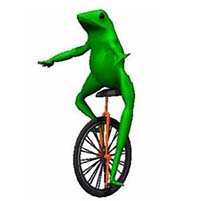
\includegraphics{DatBoi}
\end{center}
\end{figure}
}
\end{example}
}
\only<7>{
\begin{block}{Wait What?}
Note that in the example above our picture was way too big! Luckily we can control the height of pictures directy. When typing the $\backslash$includegraphics command before we type the braces \{\} by including a height or width command in brackets [].
\begin{semiverbatim}
\\includegraphics[width = WVal, height = HVal]\{foo\}
\end{semiverbatim}
\begin{itemize}
	\item The values we can give the width and height can take cm or pt (point) values. Experimentation is key to find what works best!
	\item You can also scale the image by a factor by using scale = VAL commands.
\end{itemize}
\end{block}
}
\only<8-9>{
	\begin{example}
		\only<8>{
			In my working directory I have a file named DatBoi I want to make a figure. By including the code
			\begin{semiverbatim}
				\\begin\{figure\} \newline
				\\begin\{center\}\newline
				\\includegraphics[height = 5cm]\{DatBoi\} \newline
				\\end\{center\} \newline
				\\end\{figure\}
			\end{semiverbatim}
		}
		\only<9>{
			I get the figure
			\begin{figure}
				\begin{center}
					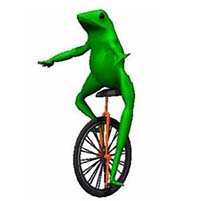
\includegraphics[height= 5cm]{DatBoi}
				\end{center}
			\end{figure}
		}
	\end{example}
}
\only<10>{
\begin{block}{Other Things with Figures}
When making figures it's also important to give captions so that we can explain what a figure does (especially since figures often don't go where we expect --- more on this later). To make captions just insert the command $\backslash$caption\{\} after you include the image in your figure as in the code below:
\begin{semiverbatim}
\\begin\{figure\} \newline
\\includegraphics\{foo\} \newline
\\caption\{A caption describing foo\} \newline
\\end\{figure\}
\end{semiverbatim}
\end{block}	
}
\only<11-12>{
\begin{example}
		\only<11>{
	In my working directory I have a file named DatBoi I want to make a figure. By including the code
	\begin{semiverbatim}
		\\begin\{figure\} \newline
		\\begin\{center\}\newline
		\\includegraphics[height = 5cm]\{DatBoi\} \newline
		\\caption\{Hey look! It's Dat Boi!\} \newline
		\\end\{center\} \newline
		\\end\{figure\}
	\end{semiverbatim}
}
\only<12>{
	I get the figure
	\begin{figure}
		\begin{center}
			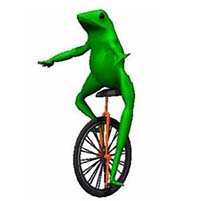
\includegraphics[height= 5cm]{DatBoi}
			\caption{Hey look! It's Dat Boi!}
		\end{center}
	\end{figure}
}
\end{example}	
}
\only<13-14>{
\begin{block}{Last Topics for Inserting Figures}
\only<13>{
While we've seen how to include figures and caption them, we still need to see how to position figures. Often \LaTeX\, will try its best to find a spot where the figure goes and fits on a page, but it will frequently become utter chaos. We won't do too much with this today save for your take home exercise, but here are the placement commands you can use in a figure as in the code below:
\begin{semiverbatim}
\\begin[PLACEMENT OPTIONS]\{figure\} \newline
foo \newline
\\end\{figure\}
\end{semiverbatim}
}
\only<14>{
The placement options are:
\begin{itemize}
	\item h: This tells \LaTeX\, to do its best to put the figure as close to the exact place relative to where you typeset the figure relative to the paragraphs around the figure as possible.
	\item !: This tells \LaTeX\, to supress finding ``good'' floats for determining where figures should go.
	\item t: This puts the figure towards the top of the page.
	\item b: This puts the figure towards the bottom of the page.
\end{itemize}
}
\end{block}	
}
\end{frame}

\section{Labels and Internal References}
\begin{frame}\frametitle{Theorem and Theorem-Like Environments}
\only<1>{
\begin{block}{We're Typesetting Books and Articles Now!}
As we do things in math (and stats? I'm displaying my ignorance here) we'll need to typeset things within theorem or proposition or lemma or definition blocks. These blocks should have numbers and labels (and proofs) so that we can refer to them and their results with cute little lines like ``by Theorem 4.20 we find the height function rises.'' Let me first show you how to make these.
\end{block}	
}
\only<2-3>{
\begin{block}{Theorem Environments}
\only<2>{
To make a theorem environment you need to define it in your preamble. This can be done via the code:
\begin{semiverbatim}
\\newtheorem\{COMMAND\}[NumberControl]\{NameToAppear\}
\end{semiverbatim}
You then call this new theorem environment by typing
\begin{semiverbatim}
\\begin\{COMMAND\}[Optional Stuff]\newline
foo\newline
\\end\{COMMAND\}
\end{semiverbatim}
}
\only<3>{
In the theorem environment COMMAND I suggested above, the NameToAppear is what appears when you call the environment. So beginning command would give you an environment like what is below. Note that by default theorem style environments italicize text like the word ``foo'' below.
}
\end{block}
}
\only<3>{
\begin{COMMAND}
	foo
\end{COMMAND}
}
\only<4-6>{
\begin{block}{Numbering Theorems}
\only<4>{
When you create a theorem environment, by default it just counts how many theorems/propositions/COMMAND/etc.\@ environments you've used in your document. It is good style to have many things number together (number theorems, propositions, lemmas, examples, and definitions together means you know roughly how far into a document a thing is; otherwise it's a crap shoot). Making this work properly just involves using that number control part when we define our environments!
}
\only<5>{
When defining multiple theorem environments, filling the number control with the name of an environment you've already defined tells \LaTeX\, to count the new environment as if it was the thing you substituted. For example, in the code
\begin{semiverbatim}
\\newtheorem\{theorem\}\{Theorem\} \newline
\\newtheorem\{lemma\}[Theorem]\{Lemma\} \newline
\\newtheorem\{Conjecture\}\{Conjecture\}
\end{semiverbatim}
every instance of lemma is counted as if it were a theorem, while Conjecture is counted separately.
}
\only<6>{
Finally, we can tell \LaTeX\, to count our theorems by order of section, subsection, or just in order of use. This is done by the command in your preamble:
\begin{semiverbatim}
\\numberwithin\{ENVIRONMENT\}\{Counter\}
\end{semiverbatim}
It tells \LaTeX\, to count each instance of ENVIRONMENT so long as the value of Counter is fixed. Some values you can feed to counter are:
\begin{itemize}
	\item section,
	\item subsection,
	\item chapter.
\end{itemize}
Note that you can also tell equations to be numberwithin'd sections as well!
}
\end{block}
}
\only<7>{
\begin{example}
Here is a preamble that will define three theorem environments with two counted independently of one and numbered by sections and chapters, respectively.
\begin{semiverbatim}
\\newtheorem\{theorem\}\{Theorem\} \newline 
\\newtheorem\{lemma\}[theorem]\{Lemma\} \newline
\\newtheorem\{FalseClaim\}\{False Claim\} \newline
\newline
\\numberwithin\{theorem\}\{section\} \newline
\\numberwithin\{FalseClaim\}\{chapter\}
\end{semiverbatim}
\end{example}
}
\only<8-9>{
\begin{block}{Definition Style  Theorem Environments}
\only<8>{
Theorem environments are great, but there is a problem: If you define a definition environment na{\"i}vely you get an italicized definition, which is not ideal. However, we can fix this by declaring that our theorem style is ``definition'' before making more new theorem environments. This is perfect for making examples and defintions and exercises (oh my)!
}
\only<9>{
Here's how to declare definition style theorems. Type something of the following nature:
\begin{semiverbatim}
\\theoremstyle\{defintion\} \newline
\\newtheorem\{def\}\{Definition\} \newline
\\newtheorem\{example\}[defn]{Example}
\end{semiverbatim}
You can even have noremal theorems defined before you say that you have $\backslash$theoremstyle\{definition\} and have both italicized and non-italicized environments!
}
\end{block}
}
\only<10>{
\begin{example}
The following code gives italicized environments (lemma, theorem) and non-italicized environments (example, definition) which all have the same counter indexed by sections:
\begin{semiverbatim}
\\newtheorem\{thm\}\{Theorem\} \newline
\\newtheorem\{lemma\}[thm]\{Lemma\} \newline
\newline
\\theoremstyle\{definition\} \newline
\\newtheorem\{defn\}[thm]\{Definition\} \newline
\\newtheorem\{example\}[thm]\{Example\} \newline
\newline
\\numberwithin\{thm\}\{section\}
\end{semiverbatim}
\end{example}
}
\only<11-12>{
\begin{exampleblock}{Exercise}
\only<11>{Write a preamble that introduces three theorem environments, two italicized and one non-italicized, that are all numbered together and indexed by sections and change the numbering so that equations are numbered within a section as well.
}

\only<12>{
Here is my sample code:
\\newtheorem\{thm\}\{Theorem\} \newline
\\newtheorem\{lemma\}[thm]\{Lemma\} \newline
\newline
\\theoremstyle\{definition\} \newline
\\newtheorem\{defn\}[thm]\{Definition\} \newline
\newline
\\numberwithin\{thm\}\{section\} \newline
\\numberwithin\{equation\}\{section\}
}
\end{exampleblock}
}
\end{frame}

\begin{frame}\frametitle{Labels and References}
\only<1>{
\begin{block}{Recall}
Before we get started remember that if you want to make an equation with a number on it like
\begin{equation}\label{Eqn: Normalized Euler}
e^{2\pi \theta} = \cos(2\pi \theta) + i\sin(2\pi \theta)
\end{equation}
is done by typing
\begin{semiverbatim}
\\begin\{equation\} \newline
foo \newline
\\end\{equation\}
\end{semiverbatim}
\end{block}
}
\only<2-3>{
\begin{block}{Labels}
\only<2>{
We now get to see how to internally reference things so that we never have to manually type in numbers that change (and, if you're using the hyperref package, can be clicked on to send you to the correct place). These are done by setting up and using labels! Luckily, setting up labels is straightforward: Immediately after your command (like a theorem environment or equation) and any options you use in it, you simply add a label:
\begin{semiverbatim}
\\begin\{thm\}[optional stuff]\\label\{DESCRIPTION\} \newline
foo \newline
\\end\{thm\}
\end{semiverbatim}
\begin{semiverbatim}
\\begin\{equation\}\\label\{DESCRIPTION\} \newline
foo \newline
\\end\{equation\}
\end{semiverbatim}
}
\only<3>{
The most important thing when writing labels is that you make your description something sensible (like naming variables in code, calling something ``fart'' is funny once but good luck searching through a zoo of ``fart1'' labels to find the correct thing you're referencing). Here are my suggestions that I use in my own code:
\begin{itemize}
	\item Begin by adding \textbf{what} you're labelling to your label. For instance, if you're labelling a theorem or lemma or equation, tell \textbf{future} you that this is a theorem or lemma or equation.
	\item Next describe roughly where this thing is (so in Section DESCRIPTION or something like that) so that you know roughly where to start looking for the thing if you need to manually check the statement of the thing it's not insane to try and find it.
	\item Finally, give a short description of what the thing actually says so you and future you know \textbf{what} you're actually referencing.
\end{itemize}
}
\end{block}
}
\only<4>{
\begin{example}
Here is a theorem environment and an equation I've labelled in an imaginary document.
\begin{semiverbatim}
\\begin\{thm\}[optional]\\label\{Thm: Section Preliminaries: Euler's Thm\} \newline
For real \\theta the equation \newline
\\begin\{equation\}\\label\{Equation: Section Preliminaries: Euler's Eqn\} \newline
e\string^\{i\\theta\} = \\cos(\\theta) + i\\sin(\\theta). \newline
\\end\{equation\} \newline
\\end\{thm\}
\end{semiverbatim}
\end{example}
}
\only<5>{
\begin{block}{References}
We now get to do the most fun thing someone can do with their labels: Referencing them! This is very easy: In your code anywhere just write $\backslash$ref\{foo\} where foo is a label you've already defined! For example:
\begin{semiverbatim}
\\begin\{thm\}[The Fart Theorem]\\label\{Thm: fart\} \newline
foo \newline
\\end\{thm\}\newline
Using Theorem \\ref\{Thm: fart\}\, we get...
\end{semiverbatim}
\end{block}
}
\only<6>{
\begin{block}{A Warning}
I just want to point out the one main thing you actually can't do with labels. You only need to make sure that each label you write is {\color{red} unique}.If your labels aren't unique \LaTeX\, will get confused and crap out.
\end{block}
}
\only<7>{
\begin{example}
Here's a theorem and equation environment with references:
\begin{semiverbatim}
\begin{semiverbatim}
	\\begin\{thm\}[optional]\\label\{Thm: Section Preliminaries: Euler's Thm\} \newline
	For real \\theta the equation \newline
	\\begin\{equation\}\\label\{Equation: Section Preliminaries: Euler's Eqn\} \newline
	e\string^\{i\\theta\} = \\cos(\\theta) + i\\sin(\\theta). \newline
	\\end\{equation\} \newline
	\\end\{thm\} \newline
	Theorem \\ref\{Thm: Section Preliminaries: Euler's Thm\}\, is classical and Equation \\ref\{Equation: Section Preliminaries: Euler's Eqn\}\, can be proved with power series tricks.
\end{semiverbatim}
\end{semiverbatim}
\end{example}
}
\end{frame}

\section{The Dreaded Beamer: Presentations in \LaTeX}
\begin{frame}
\begin{block}{The Joke's On Me}
I ran out of time. Beamer kinda sucks but the documentation on overleaf is pretty good. I've also included the source TeX for this talk in the git repo so you can dissect it and use it for your presentations.
\end{block}
\end{frame}

\section{Random Questions and Concluding Remarks}
\begin{frame}\frametitle{Any Questions?}
	
\end{frame}
\begin{frame}\frametitle{The Last Slide}
	\begin{block}{The End}
		Thanks for coming and listening everybody!
	\end{block}
\end{frame}


\end{document}